\documentclass{listhesis}
% --- Listhesis builds on KOMA script report (scrreprt).
%     Class arguments are passed to that class.

% --- Add additional packages here using \usepackage{package-name}.

% --- Provide your thesis details here.
\setup{%
  % de,                   % uncomment if your thesis is in German
  author=Iffat Brekhna, % your name
  title={Simulator Support for Dynamic Data Migration},
  date={May 21, 2018}, % submission date (today is used if unset)
  type=master,        % thesis type [master, bachelor, research, internship, diplom]
  advisor=Sven Rheindt M.Sc, % your advisor (typically some PhD. student)
  supervisor=Prof. Dr. sc. techn. Andreas Herkersdorf, % your supervisor
  % % uncomment the next lines if your thesis was carried out in industry
  % company=External Company,
  % externalAdvisor=Your Companyadvisor
}

\begin{document}

\maketitle
\cleardoublepage

% --- Thesis abstract.
%     For German thesis also provide an English version via the optional
%     argument: \anstract[English]{German}
\abstract{An abstract is defined as an abbreviated accurate
  representation of the contents of a document. -- American National
  Standards Institute (ANSI)}
\makeabstract
\clearpage

% --- Content tables.
\tableofcontents
\clearpage
\listoffigures
\clearpage
\listoftables
\clearpage

% --- Your thesis starts here.
%     Use \chapter{}, \section{}, \subsection{}, \subsubsection{},
%     and \paragraph{} to structure your thesis.

\chapter{Introduction}
This chapter serves as an introduction to the thesis. It explains the motivation for undertaking this work and the approach and concepts used in building the simulator support for dynamic data placement. Finally, the outline of the work is presented.
\section{Motivation}
Current research in semi-conductor industry is towards developing a single chip multi-tile multi-core processor. Hence, parallel programming is experiencing a rapid growth with the advent of architectures like the Invasic architecture as shown in Figure \ref{fig:multi-core,tile}. Because of multiple tiles and cores on one chip these processors deal with data processing at a high scale and complexity. Therefore, the bottleneck have shifted from computational complexities to data management capacities.\\
\\
Since modern, scalable multiprocessor system-on-chip (MPSoC) platforms have Non-Uniform Memory Access (NUMA) properties, application performance is highly influenced by data-to-task locality. The goal is to bring tasks and data closer together to increase overall performance. This is a twofold and complementary problem consisting of data and or task migration. In this thesis, we will look into data placement and see how it improves the performance of the MPSoC.\\
\\
We propose a dynamic data placement (DDP) scheme in which the data is migrated dynamically at run time from one Tile Local Memory (TLM) to another TLM if the need arises. This is the major differentiating factor of our approach, managing data placement at run time rather than at compile time.
\section{Problem}
Formerly, data placement was done statically at compile time. It is not a efficient solution since the best data location is found after running the application (trace file) once and studying its memory access pattern. Then the data is placed according to the memory access pattern and the application runs again. This is not a very realistic approach since the application has to run twice and in real life you don't know how an application will behave in the future.\\
\\
Also, in static data placement once the data is placed on TLM's that placement is fixed, you cannot change it even if the placement is having negative effects on the performance of the processor. You have to restart the application if you want to change the data placement. 
\begin{figure}[h!]
  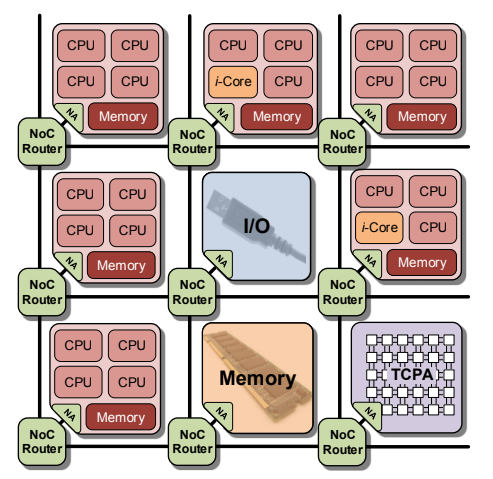
\includegraphics[width=0.5\linewidth]{multi-core,tile.png}
  \centering
  \caption{Invasic Architecture~\cite{iNetworkAdapter}}
  \label{fig:multi-core,tile}
\end{figure}
\section{Goals of Thesis}
The goal of this thesis is to design, implement and evaluate a dynamic data placement technique for memory management at run time. The system will evaluate itself and find the best data placement to improve it's performance. 
\\
The outcome will be a system which does not need external support to find the best placement for its memory but rather it will adapt itself to place the data at the best location which will in turn improve the performance. 
\section{Drawbacks}
The drawback of this thesis could be increased traffic in the processor since quite amount of data is sent back and forth in order to find the best data placement. Also, the modules used in this technique will need memory and that memory might not scale with increasing number of cores. 
\section{Approach}
The steps followed to develop the Simulator Support for Dynamic Data Migration on a Distributed Shared Memory System ... are as follows:
\begin{itemize}
  \item Understanding the Idea: In this step, the purpose is to understand why we need data migration in the first place and how data placement is done on a distributed shared memory before the application runs. We look into other means of bringing the data close to the processor as well. 
  \item Literature Review: Find and read relevant work that has already been done for bringing the data and process/task together. Choose one approach on how to bring data and task together and find relevant ideas to understanding the concept better. 
  \item Design: Here we decide which technologies to use and how to design our system for optimal results. We want a design thats easy to change, extend, optimize and is scalable. Also, we decide how we will evaluate our system eventually and what metrics we will use in result gathering. 
  \item Implementation: Implement the design of the solution. 
  \item Evaluation and Testing: Compare the results of thesis with static data placement results. --complete this after you get results iffat
  \item Writing Report: Compose a document that explains the system in detail and depict the results obtained from using this system/thesis??.
\end{itemize}
\section{Outline}
The work is structured as follows. In Chapter 1, a brief introduction of the problem is given along with the motivation to solve it and then a brief overview of the solution is given.\\
\\
In Chapter 2, the basic concepts of data migration and management along with the work already done related to this thesis is given.\\
\\
In Chapter 3, the solution/approach is explained in detail and it is shown how the solution has been implemented. \\
\\
In Chapter 4, the results are presented. It shows how the performance has changed with the proposed solution implementation. \\
\\
In Chapter 5 a summary is given and some suggestions for future works in this domain. 
\chapter{Background and Related Work}
In this chapter the necessary background information is introduced in order to understand the thesis. Moreover, we will discuss the related work in this domain of research.\\
\\
\section{Basic Concepts}
\subsection{Tile}
Figure \ref{fig:tile} shows a single tile. You can see in the figure that it composes of four CPU cores, L1 caches for every core, L2 cache which is shared between all the cores and a TLM memory which is also shared by all the cores.
\subsubsection{CPU core}
A CPU core is the basic processing unit that receives instructions(from the user or application) and performs calculations based on those instructions. A processor can have a single core or multiple cores.  
\subsubsection{TLM}
TLM stands for Tile Local Memory. Each tile has its own TLM which is shared among all the cores of the tile~\cite{ankitThesis},~\cite{iNetworkAdapter}. This memory is cachable by the L1 caches of all the cores in the tile it sits on and by the L2 cache of any other tile. The TLM from one tile can be accessed by the core of another tile.\\
\subsubsection{Cache}
Cache is a temporary storage space which is made up of high-speed static RAM (sRAM). It stores information which has been recently accessed so that it can be quickly accessed at a later time. It operates on the principle that most programs access information or data over and over again so by having data in the SRAM the CPU does not access the slow DRAM again and again. A cache hit occurs when the processor core accesses data that is already present in the cache whereas a cache miss occurs when the data is not present in the cache and has to be fetched from the TLM or the main memory to the cache~\cite{iffatseminarpaper}. In our architecture we have two levels of caches:
\begin{itemize}
  \item L1 Cache: Level 1 cache (L1 Cache) is the cache right next to the core and is the smallest in size. It is not shared with any other core i.e it is a private cache.
  \item L2 Cache:Level 2 cache (L2 Cache) is away from the processor and is larger in size than the L1 cache. It is shared between all the cores in a tile. In our scenario, L2 cache is the Last Level Cache (LLC) in the system.
\end{itemize}
\begin{figure}
  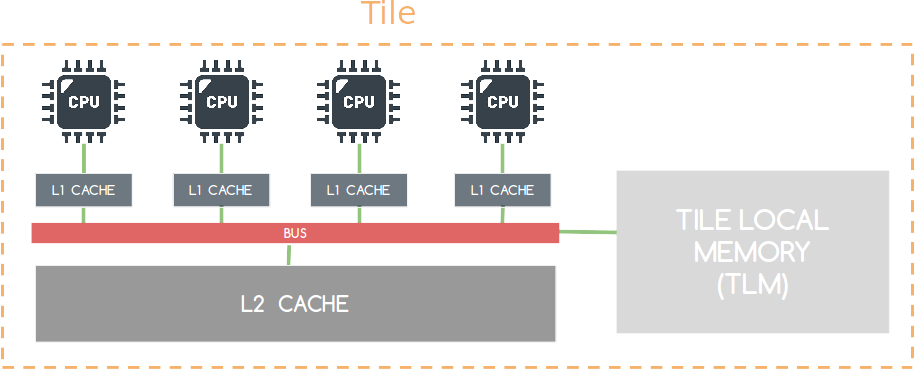
\includegraphics[width=\linewidth]{tile.png}
  \centering
  \caption{A Tile}
  \label{fig:tile}
\end{figure}
\section{Related Work}
\subsection{Data Placement/Migration on Caches}
A great amount of work have been done on data-placement in the shared last level cache in order to reduce the distance of data from the core requesting the data and to take care of load balancing across the chip.\\
\\
In static data placement~\cite{cacheDataPlacement1},~\cite{cacheDataPlacement2} the whole address space is divided into subsets and every subset is mapped to a LLC slice regardless of the location of the requesting core which leads to unnecessary on-chip traffic. Its advantage is that it evenly distributes the data among the available LLC slices and reduces off-chip accesses. In dynamic data placement~\cite{cacheDataPlacement1},~\cite{cacheDataPlacement3},~\cite{cacheDataPlacement4} the data blocks are placed such as to reduce the distance between the data block's home node and the core requesting it. This eliminates the unnecessary on-chip traffic. It requires a lookup mechanism to locate the dynamically selected home node for each data block. In reactive data placement data is classified as private or shared using the operating systems page tables at page granularity~\cite{cacheDataPlacement4},~\cite{cacheDataPlacement6}. Because all placement is performed at page granularity level there is load imbalance as some LLC slices might have higher accesses compared to others. This load imbalance leads to hot-spots~\cite{cacheDataPlacement6}.\\
\\
There is a hybrid data placement~\cite{cacheDataPlacement6} which combines the best features of static and dynamic data placement techniques. It optimizes data locality and also takes care of load balancing of the shared data. Hybrid data placement differs from Reactive data placement in regard to allocation of shared data among the cores i.e in Hybrid data placement, data is also classified as private or shared using the operating systems page tables but when a page is classified as shared (in hybrid data placement) it is allocated to a cluster of LLC slices and within this cluster the page is statically interleaved at the granularity of cache lines~\cite{cacheDataPlacement6}. This balances the load among the LLC slices.\\
\subsection{Task/Thread Placement}
Placing threads that share data on the same core improves performance~\cite{threadPlacement1}. However, finding the optimal mapping between threads and cores is a NP-hard problem~\cite{threadPlacement2} and cannot be scaled. One way to solve this problem is by monitoring the data accesses to determine the interaction between threads and the demands on cache memory~\cite{threadPlacement3}. In~\cite{threadPlacement3} a mechanism is there to transform the number of memory accesses from different threads to communication patterns and used these patterns to place the threads that share data on cores that share levels of cache.  They generate a communication matrix using the number of accesses to the same memory location by two threads and then maps the threads with highest communication to the same core. The disadvantage of this method is that generating the communication matrix through simulation is slow and they propose the application vendor provides this matrix with the application.\\
\\
In~\cite{threadPlacement4} a thread scheduling mechanism is proposed which uses the performance monitoring unit (PMU) with integrated hardware performance counters (HPCs) available in today's processors to automatically re-cluster threads online. Using HPSs they monitor the stall breakdowns to check if cross chip communication is the reason for the stalls. If that is so, they detect the sharing pattern between the threads using the data sampling feature of the PMU.  For every thread they maintain a summary vector called the shMap  which holds the signature of data regions accessed by the thread which resulted in cross-chip communication. These shMaps are analyzed i.e threads with high degree of sharing will have similar shMaps and will be placed to the same cluster. The OS then migrates the threads with higher sharing to the same cluster and place them as close as possible~\cite{threadPlacement4}.\\
\subsection{Data and Thread Migration}
In~\cite{datathreadPlacement} a mechanism called CDCS is presented which using a combination of hardware and software techniques jointly places threads and data in multi-cores with distributed shared caches. CDCS takes a multi-step approach to solve the various interdependencies. It places data first and then places threads such that the threads are close to the center of mass of their data. Then using the thread placement it again re-place the data and once again for this data it re-places the threads to get a optimum placement. This technique improves performance and energy efficiency for both thread clustering and NUCA techniques~\cite{datathreadPlacement}.\\
\subsection{Data Placement on TLM}
\subsubsection{Static Data Placement on TLM}
In static data placement the application is run twice. The first time it runs in order to find the best placement for the data and then for the second time it runs over the data placement done in the previous step. The disadvantages of this approach are that the data placement is fixed i.e even if some data block is becoming a bottleneck in performance the processor cannot migrate the memory block at rum time. It can only be changed by resetting the system. 
\subsubsection{Dynamic Data Migration on TLM}
In~\cite{dynamicPageMigration} the authors have proposed a dynamic page migration scheme for a multiprocessor architecture using point-to-point interconnects with a distributed global memory. They use the \textit{pivot} mechanism to regulate the dynamic migration of pages by keeping track of the access pattern to every local page in every distributed memory module. If the access pattern is unbalanced then the page pivots to the nearest neighbor in the direction which caused the unbalanced access pattern.\\
\\
In acquiring the results the authors assumed two sets of conditions:
\begin{itemize}
	\item infinite memory space model i.e it is assumed that the destination memory module always has free space
	\item finite memory space model i.e a page is only allowed to migrate if its destination memory module has free space
\end{itemize}
Ask Sven whether to put their results graphs here or not!
\chapter{System Architecture}
This chapter will illustrate and explain the architecture and design of the system. It will further explain each module in detail.
\section{Types of Accesses to TLM}
As mentioned in the previous chapter, figure \ref{fig:tile} depicts the inside of one tile. We have multiple such tiles in our processor hence the name multi-tile multi-core processor architecture.
\subsection{Local TLM Accesses}
Figure \ref{fig:localaccesses} depicts a scenario where a core is accessing its own tiles TLM which makes it a local TLM access. In this scenario the data transfer is happening just inside the tile and there is no traffic going outside the tile to the bus. This takes less time as data is placed close to the core that uses it. 

\begin{figure}
  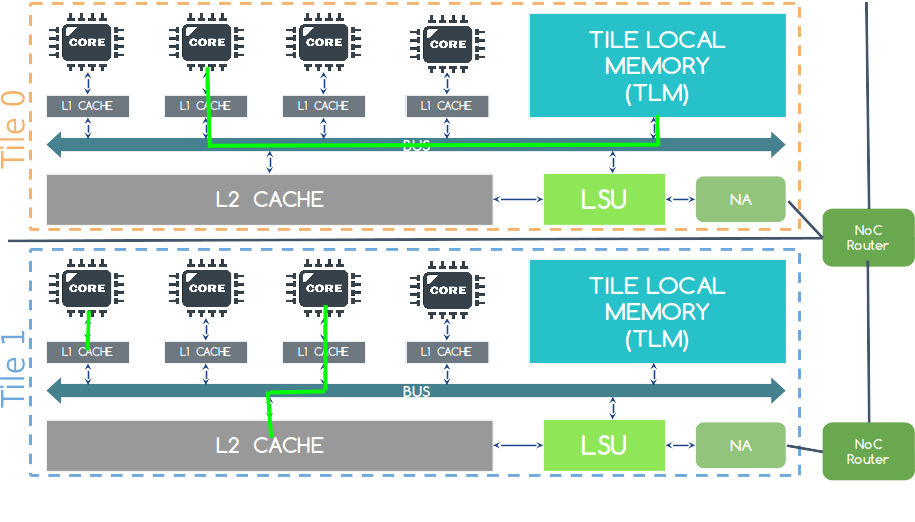
\includegraphics[width=\linewidth]{localaccesses.png}
  \centering
  \caption{A tile showing local accesses to a TLM}
  \label{fig:localaccesses}
\end{figure}
\subsection{Remote TLM Accesses}
Figure \ref{fig:remoteaccesses} depicts a scenario where a core is accessing another tiles TLM which makes it a remote TLM access. In this scenario the data transfer is happening over the bus and traffic is generated. Also, this takes more time since data is placed far away from the core that uses it. 

\begin{figure}
  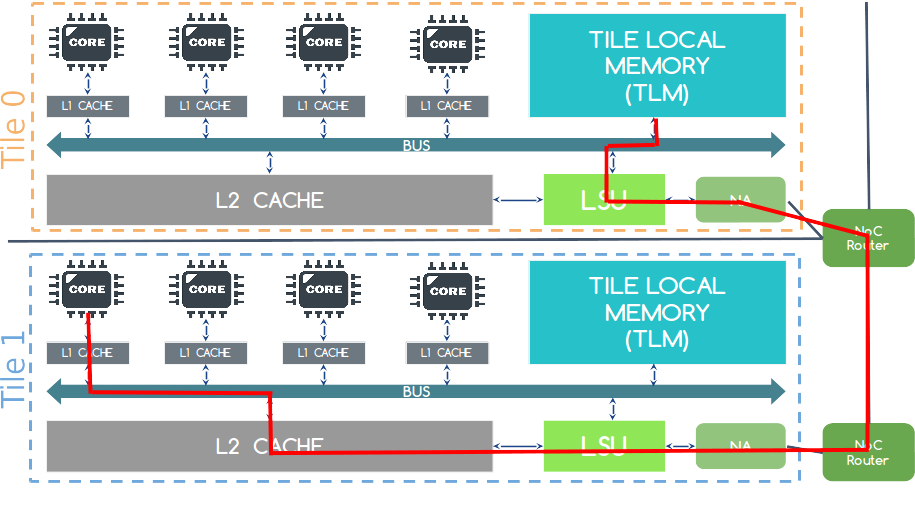
\includegraphics[width=\linewidth]{remoteaccesses.png}
  \centering
  \caption{A tile showing remote accesses to a TLM}
  \label{fig:remoteaccesses}
\end{figure}
\section{xxx}
We want to reduce the number of remote TLM accesses since it takes more time to fetch data from a TLM which is places on another tile and less time to fetch data which is on a core's own tile.  
\section{Modules Directly Used in the System for Implementing Thesis}
\subsection{Trace File}
How to explain ask from Sven! 
\subsection{Vector Address Table}
The vector address table sits between the trace file and the CPU's as shown in Figure \ref{fig:traceFile}. This table contains the address translation of all the addresses from the DRAM to the TLM. At start all TLM's are empty which means every instruction has to access data from the DRAM. The vector address table is updated if the DRAM is accessed or if migration is triggered by the central TLM Stats module and that migration takes place.
\subsection{Cache Stats Module}
The Cache{\_}Stats module is connected to the L1 and L2 Caches and is continuously getting updates from them regarding cache hits, misses, evictions etc per cache line. This module bring all the data together and at the end of the simulation prints the compulsory misses,conflict misses, evictions, local misses, remote misses, local hits, remote hits for all the caches. This module also calculates the number of local and remote access to the TLM block by using all the metrics mentioned above.
\subsection{TLM Mem Module}
This is the Tile's Local Memory and has been explained in detail in chapter 2. This module also has the functionality to observe itself and calculate whether it is empty, is full or has free space. If it has free space then it can find the staring and ending address of all the free spaces. 
\subsection{Central Stats Module}
This is the main central module which all the Cache Stats modules and TLM Mem modules are reporting to. This module is responsible of finding whether migration shall take place or not and to send out invalidation commands for the data that has to be moved in case if migration has to be triggered. 

\section{Overview/System Design}
Figure~\ref{fig:overviewOfSolution} shows the overview of the modules involved in dynamic migration scheme. Every cache module is connected to a Cache{\_}Stats module. All these Cache{\_}Stats modules and the TLM{\_}MEM modules report to the Central Stats module at every given time interval (T$_{interval}$). The central Stats module does evaluation of this data and triggers migration if needed. \\
\\
Also, the vector address table sits between the trace file and the CPU's as shown in Figure \ref{fig:traceFile}. Every instruction from the trace file first passes through the vector address table for address translation and then it is executed.

\begin{figure}[h!]
  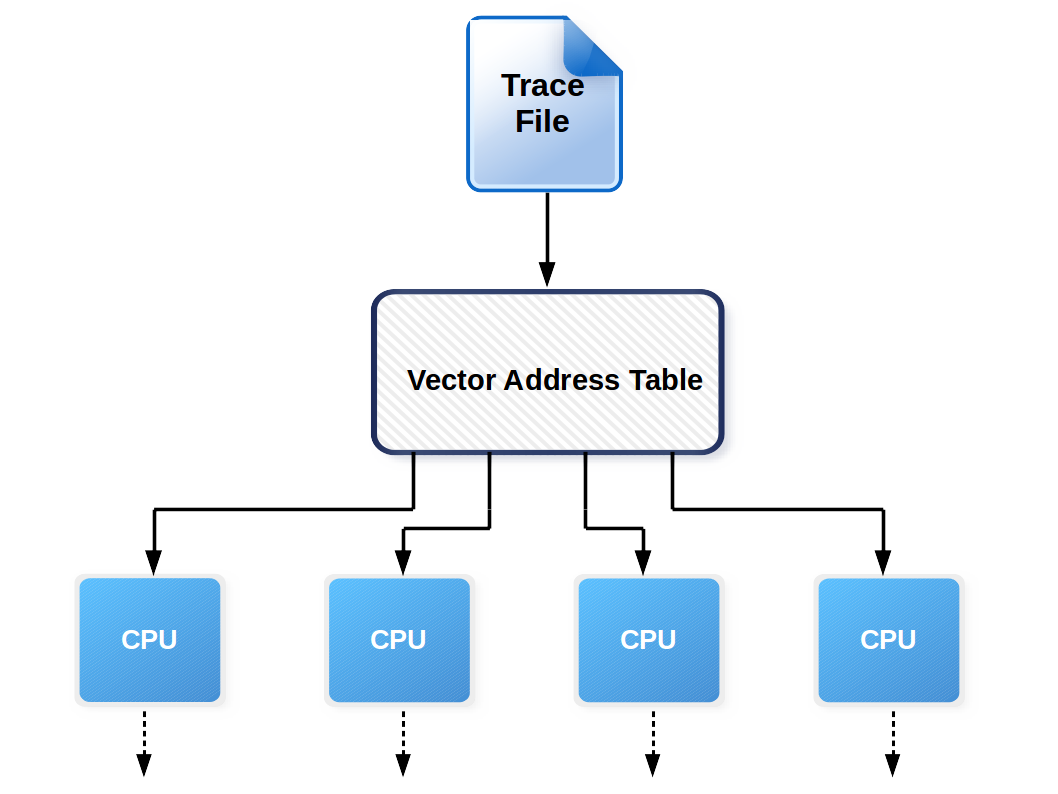
\includegraphics[width=0.7\linewidth]{traceFile.png}
  \centering
  \caption{Diagram showing where the trace file is placed}
  \label{fig:traceFile}
\end{figure}

\begin{figure}
  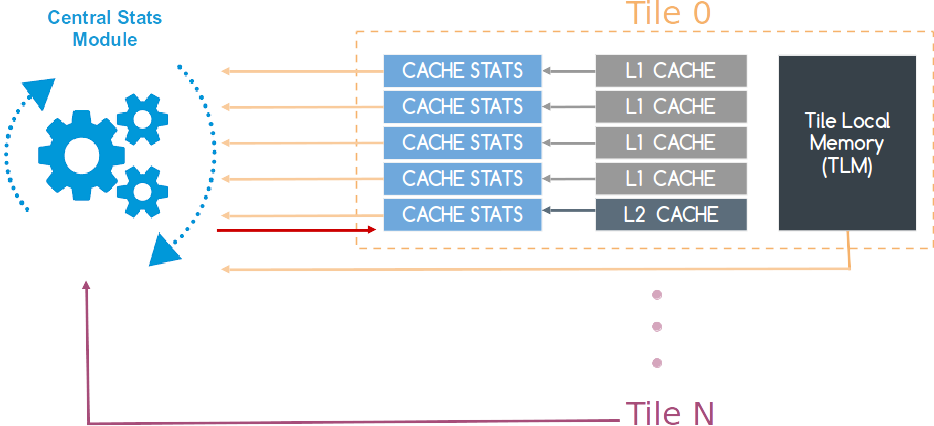
\includegraphics[width=\linewidth]{moduleconnections.png}
  \centering
  \caption{Diagram Showing Overview of the Modules Used}
  \label{fig:overviewOfSolution}
\end{figure}
\chapter{Implementation}
In this chapter, the technologies used to develop the simulator have been discussed. We further talk in detail about what how the parameters responsible for data migration are calculated and the limitations that exists in the simulator. 
\section{Tools and Technologies}

\section{Concept}
Figure \ref{fig:approachOfSolution} shows the concept of the dynamic migration scheme. It shows what messages/data are exchanged between the different modules explained/introduced above. At every given time interval (T$_{interval}$) the Cache{\_}Stats module sends the number of local and remote accesses of a TLM block to the  central TLM Stats module and the TLM{\_}MEM module sends its free address space to the central TLM stats module. This block size is equal to a number of cache lines and can be varied. The Central Stats module evaluates this data and sends a migrate command to the L2 Cache{\_}Stats module if migration shall be done.\\
\begin{figure}
  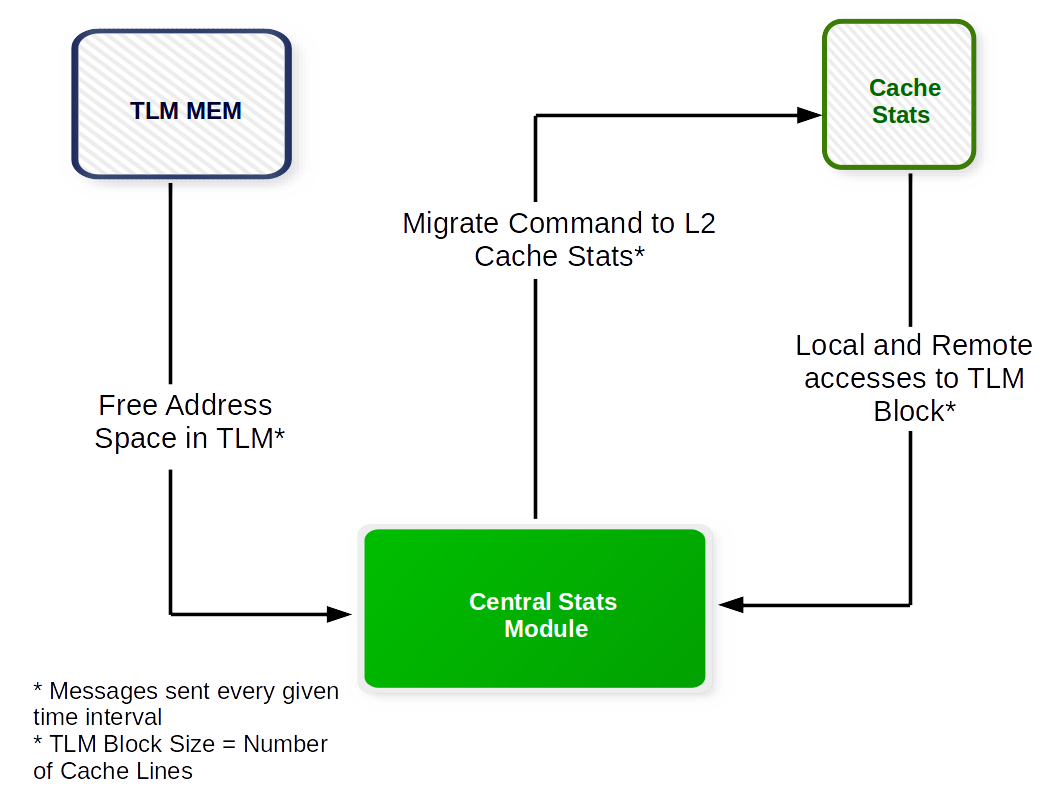
\includegraphics[width=0.7\linewidth]{approachOfSolution.png}
  \centering
  \caption{Diagram showing approach of the solution}
  \label{fig:approachOfSolution}
\end{figure}
\\
Figure \ref{fig:remoteLocalAccess} shows the how the metric for local access and remote access is calculated in the Cache{\_}Stats module. The TLM which is being accessed is compared with the current tile. If the two values are equal it means it is a request to the TLM of the same tile which means its a local access. If the two values are different it means it is a request for another tile's TLM and it is checked whether there is a L1 cache hit. If there is a L1 cache hit it means it is a local access and if it is a miss it is checked whether it is a L2 cache hit. If it is a hit it means it is a local access and if it is a miss it means it is a remote access.\\
\begin{figure}
  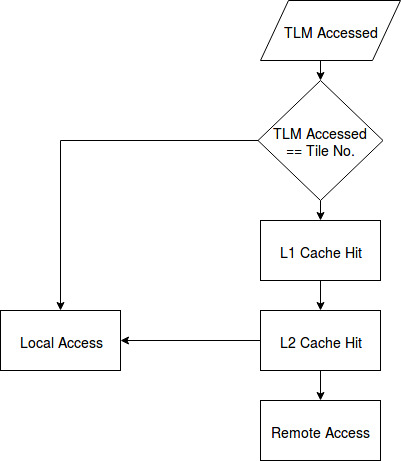
\includegraphics[width=0.5\linewidth]{remoteLocalAccess.jpg}
  \centering
  \caption{Flowchart showing process inside cache{\_}stats module}
  \label{fig:remoteLocalAccess}
\end{figure}
\\
Figure \ref{fig:freeSpaceTLM} shows how the free address space is calculated in the TLM{\_}MEM module. The vector address table is checked first and if it is empty it means all TLM's are empty. If the table is not empty and there is free space in a TLM, the starting and ending address of free space is extracted. If there is so free space in a TLM that is sent to the central TLM{\_}Stats module. \\
\begin{figure}
  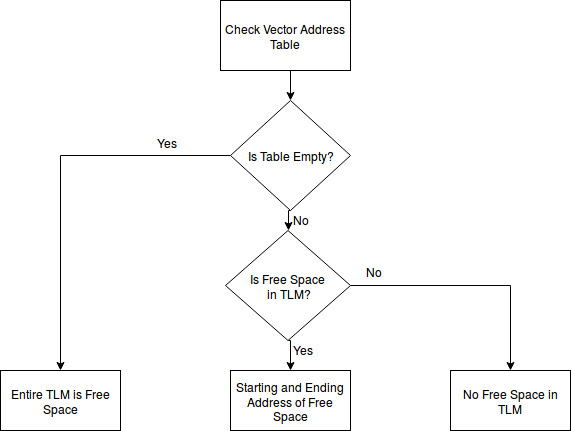
\includegraphics[width=0.7\linewidth]{freeSpaceTLM.jpg}
  \centering
  \caption{Flowchart showing how the free address space in TLM is calculated}
  \label{fig:freeSpaceTLM}
\end{figure}
\\
Figure \ref{fig:tlm_stats flowchart} shows the algorithm for determining when migration shall take place and which TLM block to migrate. First it is determined which node to migrate the TLM block to. This decision is based on the local and remote accesses to the specific TLM block. The tile with the maximum remote accesses to the TLM block is found and if these remote accesses are greater than local accesses to that TLM block it means it has to be migrated to the tile with the highest remote accesses. Then it is determined whether there is free space in the TLM of the tile to which the TLM block is to be migrated. If there is free space, a migration command is send to L2 Cache{\_|}Stats module. The migrate command is split to two commands, first reading data from the location from where data has to be migrated and then writing data at the new location. Once, the data is read a invalidation command is sent for that TLM Block/Cache Line(s) and the vector address table is updated. However, if there is no free space the block with the least number of local accesses is found in the TLM and that metric is compared with the remote accesses of the TLM block to be migrated. If the remote accesses metric is higher than the local accesses of the block with least number of local accesses a migration command is send to the L2 Cache{\_|}Stats module for this block i.e this block is migrated back to the DDR and free space is made for the incoming TLM block. Now with free space in the TLM a migration command is send to the  L2 Cache{\_|}Stats module for the block to be migrated.\\
\\
\begin{figure}
  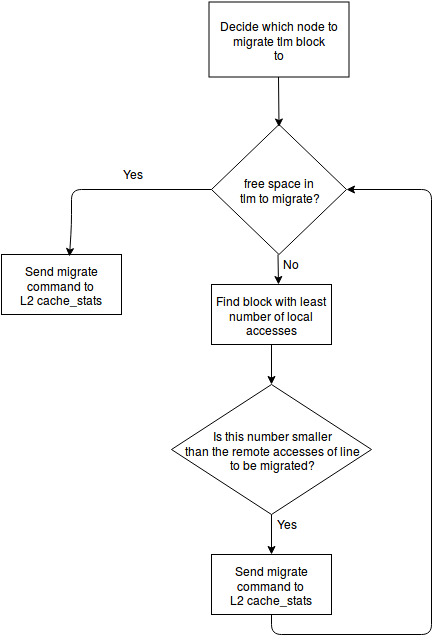
\includegraphics[width=0.7\linewidth]{tlm_stats(1).jpg}
  \centering
  \caption{Flowchart showing process inside central TLM{\_}STATS module}
  \label{fig:tlm_stats flowchart}
\end{figure}

\section{Limitations}

\chapter{Experimental Setup}
This chapter will lay out the programs that assisted in running the experiments on the Synopsys Simulator. ??Moreover, it will also illustrate the specifications of the machine that was utilized to run the experiments.
\section{Trace File}
How was the trace file generated etc...
\section{Script Runner}

\section{System Specifications}

\chapter{Evaluation}

\chapter{Conclusion and Outlook}


% --- Bibliography
\cleardoublepage
\bibliographystyle{plain}
\bibliography{thesis}

% --- Mandatory confirmation.
\confirmation

\end{document}

%%% Local Variables:
%%% mode: latex
%%% TeX-master: t
%%% End:
